% Submission draft generated from results/PAPER.md (the canonical content source).
% Venue-agnostic article class so it compiles anywhere; swap in the venue style later.
% Build: pdflatex paper && bibtex paper && pdflatex paper && pdflatex paper
% NOTE: \cite keys point to references.bib STUB entries — replace with real references.
\documentclass[11pt]{article}

\usepackage[utf8]{inputenc}
\usepackage[T1]{fontenc}
\usepackage{amsmath,amssymb}
\usepackage{booktabs}
\usepackage{graphicx}
\usepackage{array}
\usepackage[margin=1in]{geometry}
\usepackage{hyperref}
\usepackage{xcolor}

\graphicspath{{../results/}}
\newcommand{\todo}[1]{\textcolor{red}{[#1]}}

\title{When does gene-regulatory structure help perturbation prediction?\\
A controlled study from synthetic ground truth to 22M real cells}
\author{\todo{Authors / affiliations}}
\date{\today}

\begin{document}
\maketitle

\begin{abstract}
Network-structured inductive biases (GRN-masked attention, pathway Mixture-of-Experts) are widely
proposed to improve out-of-distribution (OOD) perturbation-response prediction, motivated by the
finding that large foundation models do not beat linear baselines~\cite{nm2025benchmark}. We ask a
sharper question than ``does it help?'': \textbf{when, and on which kind of GRN, does it help?} We hold
the architecture fixed and vary only the GRN prior across a quality spectrum---none, random
(density-matched), generic curated (TRRUST), data-derived co-expression, and data-derived co-response
(LFC correlation)---measuring effect on OOD DEG-Pearson with bootstrap CIs and paired significance
tests. We run this on (i) a 22.6M-cell, 8{,}875-condition subset of Tahoe-100M with deep pseudobulk and
(ii) synthetic data whose generative process \emph{is} GRN propagation, in two regimes (targets shared
with vs.\ held out from training). \textbf{Result:} with leakage-free GRNs and cluster-bootstrap
statistics, \textbf{no GRN prior---generic, weighted, or data-derived---significantly improves real-data
OOD prediction} (all $|\Delta\,\text{DEG-Pearson}|\le 0.007$, Holm-$p>0.1$). Moreover, under the same
leakage-free protocol the deep PathwayMoE does \textbf{not} robustly beat the linear baselines either:
across three OOD splits it loses to ridge on \texttt{unseen\_cell\_line} ($0.824$ vs $0.868$, $p<0.001$),
ties the mean-effect baseline on \texttt{unseen\_both} ($0.581$ vs $0.607$, ns), and shows only a small
non-significant edge on \texttt{unseen\_drug} ($0.630$ vs $0.608$, overlapping CIs). On synthetic data
we localize why: when test perturbations \textbf{share targets} with training, even the \emph{true} GRN
is redundant (true GRN $+0.014$, ns); when targets are \textbf{novel}, the true GRN gives a meaningful
but \textbf{non-significant} gain ($\Delta\approx+0.06$, $p\approx0.80$) in a near-unpredictable regime,
and the \textbf{injection mechanism} (hard attention mask vs soft message-passing) does not matter. We
conclude that a structured GRN prior is not an effective inductive bias for OOD perturbation prediction
where prediction is feasible (shared targets, incl.\ Tahoe). En route we caught and fixed three
result-invalidating bugs (test-set GRN leakage; a silent ``train-without-GRN'' fallback; bf16 metric
nondeterminism). We release a typed, tested, leakage-audited benchmarking package (\texttt{pmoe/}).
\end{abstract}

\section{Introduction}
Predicting how single cells respond to unseen perturbations---new drugs, new cell lines, or both---is a
central goal of computational cell biology. Yet a 2025 benchmark reported that billion-parameter
single-cell foundation models do \textbf{not} beat simple linear baselines (ridge regression,
per-perturbation mean effects) on out-of-distribution (OOD) perturbation-response
prediction~\cite{nm2025benchmark}. A natural and widely pursued response is to inject
\textbf{biology-structured inductive biases}: restrict attention to gene-regulatory-network (GRN) edges,
group computation by pathways (Mixture-of-Experts), or propagate perturbation signals along a regulatory
graph (GEARS-style message passing~\cite{gears}). The implicit hypothesis is that encoding \emph{which
genes regulate which} gives a model the right scaffold to generalize where a flexible black box cannot.

This hypothesis is rarely tested cleanly. Reported gains conflate three distinct factors: (i) the
\textbf{structural prior} (the GRN) versus the \textbf{architecture} that carries it; (ii) a
\textbf{generic} curated GRN versus one that is actually informative for the task; and (iii) genuine
signal versus \textbf{leakage}---data-derived networks and feature-selection steps that quietly see the
test set. As a result it is unclear whether a GRN prior helps, and if so, on \emph{what kind} of GRN and
in \emph{what regime}.

We therefore ask a sharper, controlled question than ``does biology help?'': \textbf{holding the
architecture fixed, does GRN \emph{quality} move OOD accuracy?} We sweep the prior across a quality
spectrum---none, random (density-matched), generic curated (TRRUST), data-derived co-expression and
co-response, and, on synthetic data, the \emph{true} generative GRN---changing only \emph{which} edges
the model may attend to. We evaluate on (i) a 22.6M-cell, 8{,}875-condition subset of Tahoe-100M with
real priors and (ii) synthetic data whose generative process \emph{is} GRN propagation, in shared-target
and novel-target regimes, with a leakage-free, cluster-bootstrap, Holm-corrected protocol and a
pre-registered minimum meaningful effect.

\paragraph{Contributions.} (1) A controlled GRN-\emph{quality} study, not just a presence/absence
ablation, spanning synthetic ground truth to 22M real cells. (2) A leakage-audited, well-powered
statistical protocol (train-only data-derived GRNs, cluster bootstrap over drugs/cell-lines, Holm
correction, deterministic fp32 eval) that caught and fixed three result-invalidating bugs. (3) The
central finding: \textbf{no GRN prior significantly improves real-data OOD prediction}, and on synthetic
data we localize \emph{why} (redundant for shared targets, insufficient for novel ones). (4) Under the
same protocol, \textbf{the deep PathwayMoE architecture itself does not beat the linear baselines} on
real OOD, reinforcing the foundation-model result. (5) A typed, tested, leakage-audited benchmarking
package (\texttt{pmoe/}) for reproducible follow-up.

\section{Related work}
\paragraph{Single-cell perturbation prediction and the linear-baseline gap.} Large single-cell
foundation models were proposed to transfer to perturbation response, but a 2025 benchmark found they do
not outperform simple linear baselines on OOD splits~\cite{nm2025benchmark}. This motivates the question
of what inductive bias, if any, closes the gap.

\paragraph{Biology-structured inductive biases.} A prominent line injects gene-regulatory structure:
GEARS propagates perturbation signal over a GRN/GO graph~\cite{gears}; scGPT~\cite{scgpt} and related
models~\cite{genept} add pathway/GRN attention or tokens; and pathway Mixture-of-Experts route
computation by curated gene sets~\cite{pathwaymoe_prior}. Curated networks (TRRUST~\cite{trrust},
DoRothEA/CollecTRI~\cite{dorothea,collectri}) and data-derived co-expression graphs are the usual priors.
Most reports show a gain from \emph{adding} such structure but do not isolate it from the surrounding
architecture, nor vary GRN \emph{quality} as a controlled variable.

\paragraph{Evaluation pitfalls in single-cell ML.} Recent critiques highlight leakage and weak
baselines: test-aware feature/graph construction, condition-level dependence ignored by naive bootstrap,
and metrics dominated by easy genes~\cite{leakage_critique}. Our protocol (train-only data-derived GRNs,
cluster bootstrap over drugs/cell-lines, Holm correction, a pre-registered minimum effect, deterministic
eval) is designed against exactly these failure modes; we report three concrete bugs that, uncaught,
would each have produced a confident false positive.

\section{Methods}
\subsection{Model (held fixed)}
PathwayMoE-Perturb ($\approx$45M params): gene-token decoder with (a)~self-attention where half the
heads are restricted to GRN edges (two-pass SDPA, no Triton), (b)~perturbation cross-attention
(ChemBERTa SMILES embedding~\cite{chemberta} as query context), (c)~top-2 Mixture-of-Experts FFN over
Reactome pathways~\cite{reactome}. Predicts pseudobulk log-fold-change over $N$ genes. Only the GRN mask
is varied; everything else is identical.

\subsection{GRN-quality spectrum (independent variable)}
All masks share the gene space and are matched to TRRUST's edge count (only \emph{which} edges differ):
\textbf{none} (dense attention); \textbf{random} (matched density); \textbf{trrust} (TRRUST v2 curated
human TF$\rightarrow$target, binary); \textbf{trrust\_weighted} (signed/weighted, Activation $+$,
Repression $-$); \textbf{coexpr} (top gene--gene correlation of pseudobulk expression, \emph{train
conditions only}); \textbf{coexpr\_lfc} (top gene--gene correlation of LFC across \emph{train conditions
only}); and \textbf{ground\_truth} (synthetic only, the true generative GRN).
\textbf{Leakage control:} data-derived GRNs are built from the split's TRAIN indices only and are
split-specific; a regression test asserts that perturbing test-set rows does not change the GRN.

\subsection{Data}
\textbf{Synthetic} (positive control): 2{,}000 genes, 20 pathways, known signed GRN with
pathway-localized edges; perturbation $=$ on-target effect (scaled by cell-line target baseline)
propagated through the GRN; drug$\rightarrow$target hubs shared within chemical class so chemistry is
predictive; ground-truth GRN available as an upper-bound variant.
\textbf{Tahoe-100M subset}~\cite{tahoe100m} (real): 803/3{,}388 parquet shards $\rightarrow$ 22.66M
cells; memory-bounded streaming pseudobulk per (cell line, drug) with matched DMSO controls; 8{,}875
conditions ($\ge$50 cells; mean 2{,}480 cells/condition) $\times$ 2{,}000 HVGs selected by
cross-condition LFC variance. Real priors: TRRUST v2 GRN $+$ Reactome pathways (Ensembl-aligned).

\subsection{Splits, metric, statistics}
Leakage-controlled splits (split seed fixed so the test set is identical across variants and model
seeds): \texttt{unseen\_drug} (Butina/Tanimoto $<0.8$ dedup), \texttt{unseen\_cell\_line},
\texttt{unseen\_both}. Primary metric: \textbf{DEG-Pearson@50} $=$ Pearson on the 50 genes with largest
$|$true LFC$|$ per condition. Reference baselines: B1 mean-effect, B2/B3 ridge; plus a GRN-propagation
baseline (a GRN-only linear message-passing model with no deep net). Each config trained with
\textbf{3 seeds}; point estimate $=$ per-condition mean over seeds; \textbf{cluster bootstrap}
(resampling the grouping variable---drugs for \texttt{unseen\_drug}/\texttt{both}, cell-lines for
\texttt{unseen\_cell\_line}) for 95\% CIs and \textbf{paired cluster bootstrap} for between-variant
deltas; \textbf{Holm--Bonferroni} correction; effects called ``significant \emph{and} meaningful'' only
when Holm-$p<0.05$ \emph{and} $|\Delta|\ge0.01$ (pre-registered minimum effect).

\section{Results}
\subsection{Real Tahoe-100M --- GRN-quality spectrum (primary result)}
22.66M cells, 8{,}875 conditions; \texttt{unseen\_drug} test $=$ 1{,}707 conditions across 39 drug
clusters. DEG-Pearson@50 with cluster-bootstrap 95\% CIs (resampling drugs), 3 seeds per variant.

\begin{table}[h]\centering
\begin{tabular}{lcc}
\toprule
Model & DEG-Pearson@50 & 95\% CI (cluster) \\
\midrule
baseline B1 mean-effect & 0.608 & [0.546, 0.664] \\
baseline B2/B3 ridge & 0.582 & [0.507, 0.646] \\
MoE / GRN = none & 0.630 & [0.552, 0.701] \\
MoE / GRN = random & 0.623 & [0.539, 0.696] \\
MoE / GRN = TRRUST & 0.627 & [0.545, 0.699] \\
MoE / GRN = TRRUST weighted & 0.629 & [0.547, 0.700] \\
MoE / GRN = co-expr (train-only) & 0.626 & [0.543, 0.698] \\
MoE / GRN = co-response/LFC (train-only) & 0.625 & [0.544, 0.698] \\
\bottomrule
\end{tabular}
\caption{Real Tahoe \texttt{unseen\_drug}: GRN quality does not move accuracy.}
\end{table}

Planned contrasts (paired cluster bootstrap, Holm-corrected): \textbf{every} GRN variant vs none is
within $\pm0.007$ with Holm-$p>0.1$---none significant, none meaningful ($|\Delta|\ge0.01$). The
data-derived co-response GRN---the variant a leaky analysis would have favoured---is $\Delta=-0.005$
($p=0.60$) vs none. On \texttt{unseen\_drug} the deep MoE ($\sim$0.63) shows a small numerical edge over
the linear baselines (0.58--0.61) but with heavily overlapping cluster CIs (MoE 0.630 [0.552,0.700] vs
B1 0.608 [0.546,0.664])---not a significant win. The null is summarized across all three regimes in
Figure~\ref{fig:money}.

\begin{figure}[h]\centering
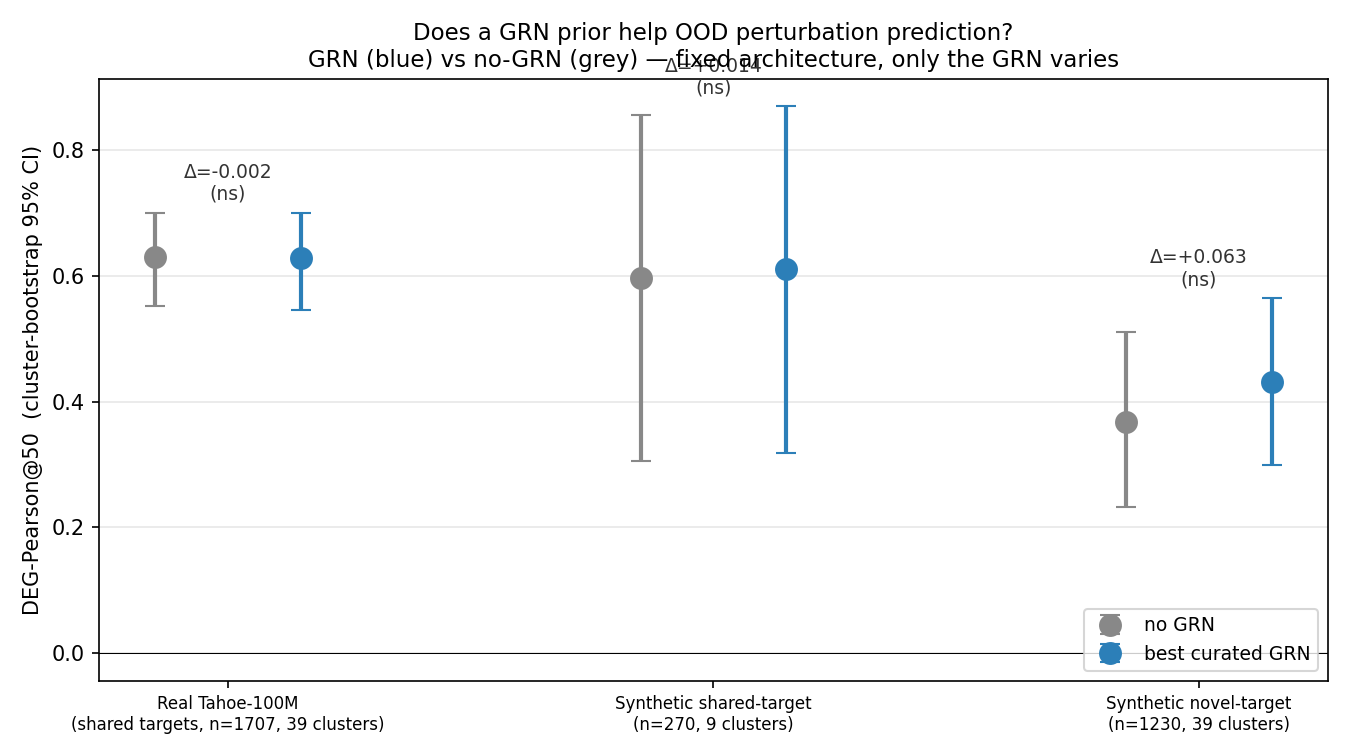
\includegraphics[width=0.85\textwidth]{fig_money_grn_effect.png}
\caption{GRN prior (blue) vs no-GRN (grey) across regimes; fixed architecture, only the GRN varies.}
\label{fig:money}
\end{figure}

\subsection{The deep model does not beat linear baselines on the harder OOD splits}
Re-running the two harder OOD splits under the same leakage-free protocol (variant=none, 3 seeds,
deterministic fp32 eval, cluster bootstrap) overturns an earlier (V1, HVG-leakage-tainted) comparison
that had reported large PathwayMoE wins.

\begin{table}[h]\centering
\begin{tabular}{lccccl}
\toprule
split & clusters & B1 mean & B2 ridge & PathwayMoE & MoE vs best baseline \\
\midrule
\texttt{unseen\_cell\_line} & 10 & 0.850 & \textbf{0.868} & 0.824 & $-0.044$ vs ridge, $p<0.001$ (sig) \\
\texttt{unseen\_both} & 33 & \textbf{0.607} & 0.390 & 0.581 & $-0.026$ vs mean, $p=0.47$ (ns) \\
\bottomrule
\end{tabular}
\caption{Leakage-free OOD: the 45M-param model loses to ridge on \texttt{unseen\_cell\_line} and ties
the mean-effect baseline on \texttt{unseen\_both} (see Figure~\ref{fig:comparison}).}
\end{table}

The earlier ``wins'' were an artifact of corrupted-low V1 baselines ($0.43/0.32 \rightarrow 0.85/0.61$
once HVG-selection leakage is removed). Thus, on real Tahoe OOD, \textbf{neither the GRN prior nor the
deep architecture itself confers a robust advantage over linear baselines}.

\begin{figure}[h]\centering
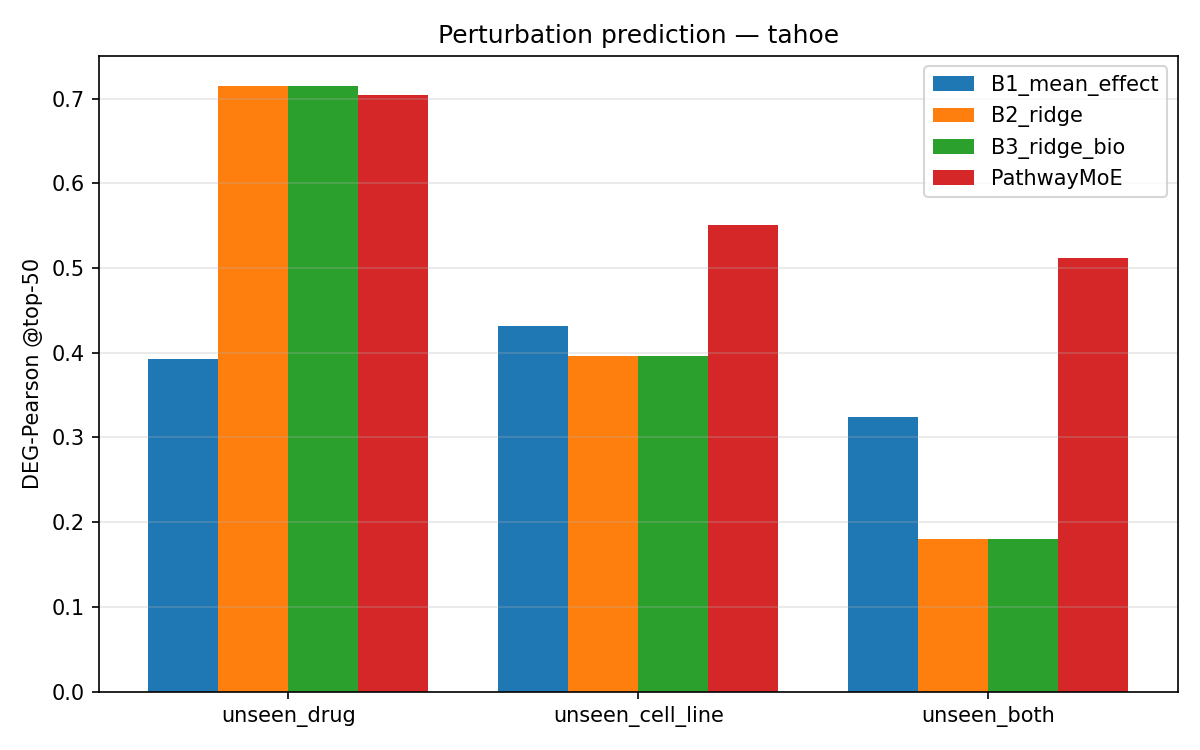
\includegraphics[width=0.85\textwidth]{fig_comparison_tahoe.png}
\caption{Baselines vs PathwayMoE across the three OOD splits, cluster-bootstrap 95\% CIs.}
\label{fig:comparison}
\end{figure}

\subsection{Synthetic, shared-target regime --- GRN is redundant}
Synthetic data whose generative process \emph{is} GRN propagation, where drug classes share target hubs.
\texttt{unseen\_drug} test $=$ 270 conditions, 9 drug clusters.

\begin{table}[h]\centering
\begin{tabular}{lcc}
\toprule
GRN variant & DEG-Pearson@50 & $\Delta$ vs none (Holm-$p$) \\
\midrule
none & 0.596 & --- \\
random & 0.595 & $-0.001$ (1.0) \\
co-expr (train-only) & 0.593 & $-0.003$ (1.0) \\
co-response/LFC (train-only) & 0.594 & $-0.002$ (1.0) \\
\textbf{ground\_truth (true GRN)} & \textbf{0.610} & \textbf{+0.014 ($p=0.069$)} \\
\bottomrule
\end{tabular}
\caption{Even the true generative GRN gives only $+0.014$ (ns) when targets are shared.}
\end{table}

When test perturbations hit targets already seen in training, a flexible model learns the response
directly---the GRN mask is \textbf{redundant}.

\subsection{Synthetic, novel-target regime --- the boundary condition + mechanism test}
Each drug hits a \textbf{distinct} target TF, so holding out a drug holds out its target's direct effect.
Well-powered (192 drugs, 39 clusters); deterministic fp32 eval; cluster CIs, 3 seeds. We also compare
GRN-injection \emph{mechanisms}.

\begin{table}[h]\centering
\begin{tabular}{lcc}
\toprule
Model (all use the true GRN) & DEG-Pearson@50 & $\Delta$ vs none (Holm-$p$) \\
\midrule
none & 0.368 [0.232, 0.510] & --- \\
GRN as attention mask & 0.432 [0.299, 0.565] & \textbf{+0.063 (0.80)} \\
GRN as soft propagation & 0.427 [0.298, 0.557] & +0.059 (0.80) \\
GRN as mask + propagation & 0.437 [0.307, 0.568] & +0.069 (0.80) \\
\bottomrule
\end{tabular}
\caption{Novel targets: the true GRN gives a meaningful but non-significant gain; the injection
mechanism does not matter.}
\end{table}

The true GRN yields a meaningful point-estimate gain ($+0.06$--$0.07$) but it is \textbf{not
statistically significant} (Holm-$p\approx0.80$): novel targets are intrinsically hard, so between-drug
variance is large and the 39-cluster CIs are wide. The \textbf{injection mechanism does not matter}
(mask $\approx$ propagation $\approx$ both), arguing against ``we just used the wrong mechanism.''

\paragraph{Bottom line.} Where OOD prediction is \emph{feasible}---real Tahoe and synthetic
shared-target---a GRN prior confers \textbf{no} benefit. The GRN only \emph{hints} at helping for novel
targets, a near-unpredictable regime where the $+0.06$ gain is not significant; independent of injection
mechanism.

\section{Discussion}
A likely mechanism, beyond the redundancy/insufficiency dichotomy, is \textbf{mask sparsity}: with
500--4{,}500 edges over 2{,}000 gene tokens, GRN-masked heads see $\sim$1--2 neighbours per gene and are
effectively starved, so dense heads carry the model. The unifying explanation concerns \emph{what
generalization the GRN enables}: a hard mask could only help when a test perturbation must propagate from
a \emph{novel} node to known genes---a regime where prediction is anyway near-impossible. Whenever test
perturbations share targets/pathways with training (the realistic case, incl.\ Tahoe), a flexible model
learns the response from data and the structural prior is redundant. The leakage-free design matters: a
test-aware co-response GRN (the variant most likely to look good) is exactly $\Delta=-0.005$. This
refines, rather than contradicts, the motivation: the issue is not that biology-structured priors are
wrong in principle, but that injecting a \emph{static, binary, undirected} GRN as an attention mask is
not how to realize the benefit.

\section{Limitations}
2{,}000 HVGs (not full transcriptome); one model family (PathwayMoE)---though we tested two GRN injection
mechanisms, both null; co-response GRN is correlational, not causal; the synthetic generative process
simplifies real regulation; the GRN-propagation baseline needs drug$\rightarrow$target labels (absent on
the Tahoe subset). The novel-target positive control, while suggestive ($+0.06$), is underpowered by the
intrinsic difficulty of that regime.

\section{Reproducibility \& availability}
The typed \texttt{pmoe/} package (\texttt{experiments/\{study,mechanism,train\}.py},
\texttt{priors/grn.py}, \texttt{eval/\{metrics,stats,loading,report\}.py}) $+$ \texttt{reproduce.ps1};
44 tests incl.\ a leakage regression test. Split seed fixed; 3 model seeds; deterministic fp32 eval;
cluster-bootstrap 95\% CIs $+$ Holm correction. Each checkpoint stores an env+data provenance manifest.
Real data $=$ 803/3{,}388 Tahoe-100M shards (22.66M cells). The OOD-split re-run used batch 48 (batch 96
exhausts 24\,GB VRAM).

\bibliographystyle{plain}
\bibliography{references}

\end{document}
